\chapter{Literature Survey}

Automatic Speech Recognition on music is a barely topic, since the applications on it are mostly for entertainment. Moreover, even though the research of ASR on music are small in quantity, most of them focus mainly on lyrics alignment not lyrics transcription over last decades. However, the continuous researches on music transcription come out since 2010, published by Messaros and Virtanen\cite{Reference5}. 
In terms of lip-reading, the first end-to-end model in the world based on Neural Networks called LipNet\cite{Reference6} comes out in 2016. It maps a variable-length sequence of video frames to text that called sentence-level lip-reading. No one can deny that it is am important breakthrough in lip-reading.
And when it turns to lip-reading for song transcription, the materials that we can find are less. In order to have a basic understanding on how to build an AV-ASR system for song transcription, this Chapter would cover the literature survey on three main component : the methods of extracting audio and video features, two kinds of classification methods (GMM-HMM basically and DNN) and HMM-GMM based ASR system in music. At last, the issues on datasets and a chapter summary are also following concludes.

\section{Feature Extraction }

Feature extraction is a vital stage in our HMM-GMM based ASR systems. To extract useful feature, we avoid any meaningless features, repeated features and complicated features in principle. And try to find a suitable set with the least dimensional feature vectors to achieve the best estimation. Because low dimensional data consumes less machine computing time and also simplifies the training model. If we get a lot typical feature vectors and train a very complicated model, the training error would decrease on training set. But for the testing error, it would increase along with the rise of the complexity of training models. Therefore, how to extract feature and what kind of feature to extract has a fatal impact on system evaluation.
And in this section, we will emphasize the process and methods of extracting both audio and video features.

\subsection{Audio Feature Extraction}
This section is to describe how to get the acoustic feature factors that transformed from the input waveform. And in this feature extracting process, we would particularly make research on MFCC \cite{Reference7}(the mel frequency cepstral coefficients, a widely used feature representation in speech recognition) and use scripts in Kaldi to realize to get the feature vectors. And here is the figure \ref{fig:mfccpro} to describe the extracting process.
\begin{figure}[ht]
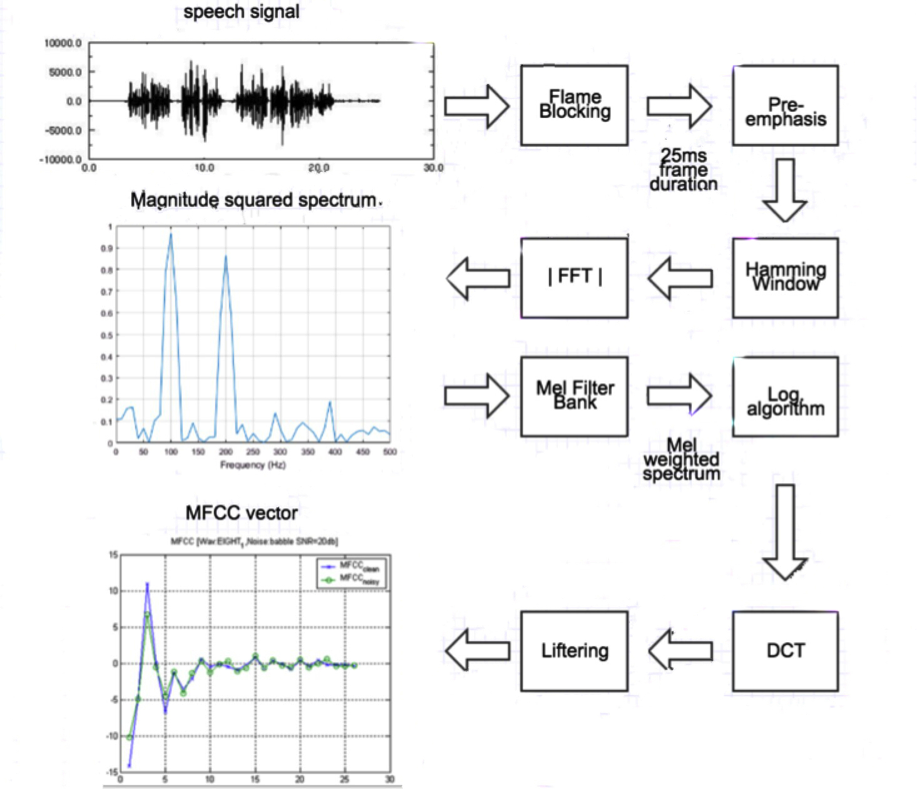
\includegraphics[width=1\linewidth]{figures/extractmfccprocess.png}
\caption{the process of extracting mfcc feature vectors}
\label{fig:mfccpro}
\end{figure}


As the figure shows above, we can conclude the process of extracting mfcc feature vectors into several steps:
\begin{enumerate}
\item Sample and quantize the speech signal into digital waveforms.
\item Frame blocking typically 25 ms frames duration with 10ms shift.
\item Boost the waveforms’ energy in the part of high frequencies by using a high-pass filter. 
\item Use Hamming window to make frames continuous for Fourier analysis.
\item Adapt FFT algorithm to compute the DFT in order to get the spectrum from hamming-windowed signal.
\item Collect energy from each frequency band by Mel filter bank and get fbank feature.
\item Compute the log of the spectrum values in each Mel bin.
\item Take the DCT and keep as many as MFCC coefficients.
\item Do cepstral liftering to scale the range of coefficients.
\end{enumerate}
In this way, we can get standard cepstral vectors of audio. To extract dynamic mfcc features, we do delta function on mfcc to get the velocity of feature changes. Besides, if we adapt delta-delta function on mfcc, we can get accelerated velocity of feature variation .



\subsection{Visual Feature Extraction}
Visual feature can be divided as appearance-based pixel feature and shape-based feature. And in our visual-only ASR system, we use the ensemble regression tree method\cite{Reference8},which is implemented in dlib toolkit to extract histogram of oriented gradients feature\cite{Reference9} in order to detect facial 68 landmarks feature. And then we extract the according to the lip region landmarks. Here the histogram of oriented gradients feature is shape-based feature, while lip region pixel feature is appearance-based pixel feature.

Nowadays, the methods of extracting video features are mainly based on pixels or models. And this section would focus on means of models, especially on the literature of ASM and AMM, since they have been proved more informatively and visually on extracting facial features with flexible and repeated geometrical characteristic.

\subsubsection{Active Shape Models}
Active shape models (ASMs)\cite{Reference10} are statistical models of the shape of objects, which aims to fit an example of the same object in a new image by iteratively deform. ASMs are models generally consist of two parts: A Point Distribution Model and a set of Local Gray-Level models. The former part uses object’s landmark points to model the shape and its variants. Besides, the latter part is used to capture the local gray-level variants at each landmark points. 

ASMs are also flexible models to represent the shape and appearance of faces in images. It uses Principal Component Analysis\cite{Reference11} (PCA) to learn a generic model from the facial landmarks in training data, and then fits the best match target points in test data, typically by some greedy searches.

Here are also some ASM fitting result \ref{img:ASM1} show below, which gets by initializing an approximate fit to the training data, and then updating the parameters (Xt, Yt, s, θ, b), applying constraints to them and repeat until convergence.

\begin{center}
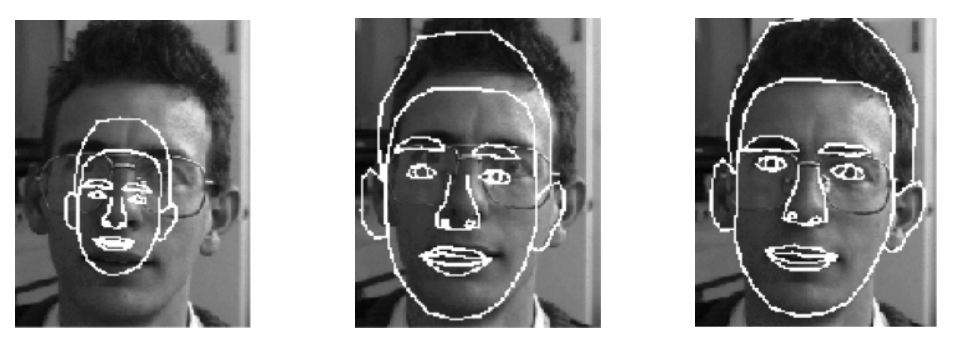
\includegraphics[width=0.8\linewidth]{images/ASM1.png}\\[1cm]
\label{img:ASM1}
\end{center}

\subsubsection{Active Appearance Model}


An active appearance model \cite{Reference12}(AAM) is a computer vision algorithm combined a statistical shape model with a texture model that aims to match a set of object shape and appearance to a new image. It is related to the ASM, since they have similar process to build models from training phrase. The difference is that the ASM seeks to match model points, while the AAM seeks to match not only the model points but also a representation of the texture of the object in an image. Therefore, the AAM can be considered as an extension of the ASM approach and be used in object detection widely nowadays. In our project, we can use tools like dlib or openCV to get the object’s shape and texture information in image, and then fits the best match model in testing data, typically by some greedy searches. 

Compared with ASM,our project is more reasonable to adapt AAM,since it learns model from both shape and texture information, while sometimes singer does not face to the camera. As a result, tools may be not get the landmarks. Problems get solved when adapting AMM rather than ASM.

Applying PCA, we can model the statistical variation with formula below.
        
        A shape model:
        \begin{equation} X=\bar{X}+P_{s}b_{s}\end{equation}
        A texture model:
        \begin{equation}  g=\bar{g}+P_{g}b_{g}\end{equation}
        A shape and texture combined model:
        \begin{equation}  
       b=\begin{pmatrix}
W_{s}b_{s}\\b_{g}
\end{pmatrix}=\begin{pmatrix}
W_{s}P_{s}^{T}(x-\bar{x})\\ P_{g}^{T}(g-\bar{g})
\end{pmatrix}
        \end{equation}
        
Here are some examples to show the AAM fitting result\ref{img:AAM1}.
\begin{center}
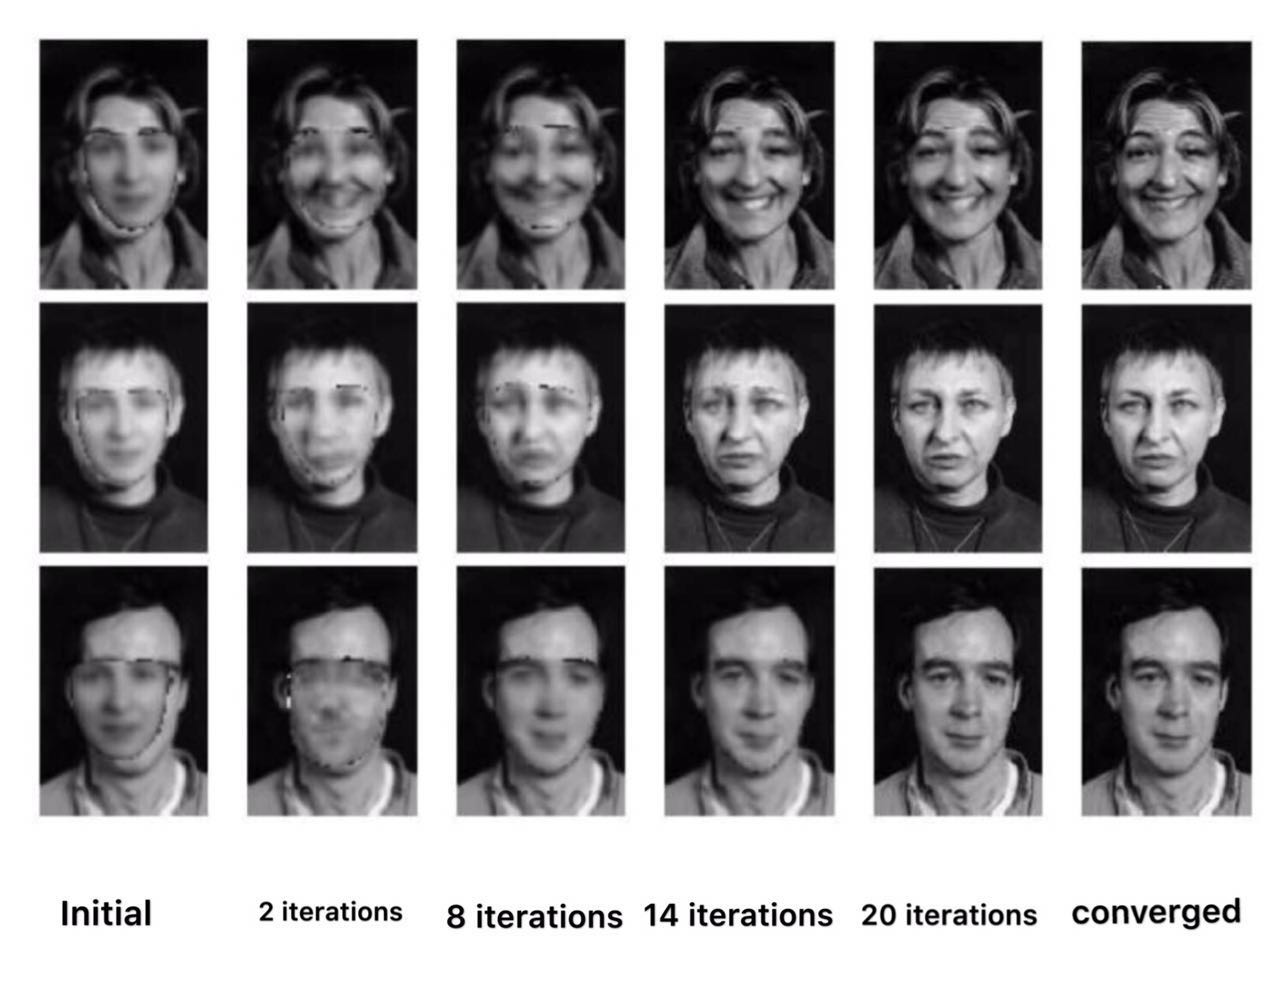
\includegraphics[width=0.8\linewidth]{images/AAM1.jpeg}\\[1cm]
\label{img:AAM1}
\end{center}

\subsubsection{Audio-Visual fusion}
Audio–visual fusion is a major research topic in the process of building an AV-ASR system, which aims to combine video with audio streams into a bimodal classifier. The video streams are usually starts early than audio streams, for example when the lip starts to move, the voice still not come out. Since the two streams are not perfectly synchronous with each other, the AV-fusion is complicated.

Basically, we have two methods that can be considered for AV-fusion: feature fusion, decision fusion. Feature fusion is considered as an “early” level fusion method, while decision fusion is a “late” level fusion\cite{Reference13}. Even though feature fusion techniques making work easier in improving ASR over audio-only result, the reliability of each modality cannot be ensured. Therefore, using a weighted decision fusion to develop the AV-ASR system may get better results than using feature level fusion. However, the decision fusion may be more difficult than feature fusion.

\section{Classification}
In this section, we would cover the literature of statistic models, HMM and GMM. They are popular models to be adapted into ASR systems. Since we did not adapt DNN methodologies into our system, the literature on DNN we covered in the chapter is rough. It is for introduction, because using the machine deep learning methodology is the new trend to develop ASR systems.

\subsection{Gaussian Mixture Models}
The Gaussian Mixture Model \cite{Reference14}(GMM) is a most common parametric probability density function by far, which superposed by M component Gaussian densities, to describe the distribution of the dataset.
At the same time, a GMM can be expressed by equation (2.4) in a mathematical way. 

\begin{equation}
p(x|\lambda )=\sum_{i=1}^{M}w{_{i}}g(x|\mu{_{i}},\Sigma _{i} )
\end{equation}

where, \begin{equation}
\sum_{i=1}^{M}w{_{i}}=1
\end{equation}
  (x is a D-dimensional vector data, wi , i = 1, . . . , M, are the weights for every single Gaussian function)
The shape of Gaussians controlled by the mean and unit variance,  
Gaussians have the same shape, with the location controlled by the mean, and here is the figure \ref{fig:gmm} to show the shape of one-dimensional Gaussians with different mean and variance.

\begin{figure}[ht]
\centering
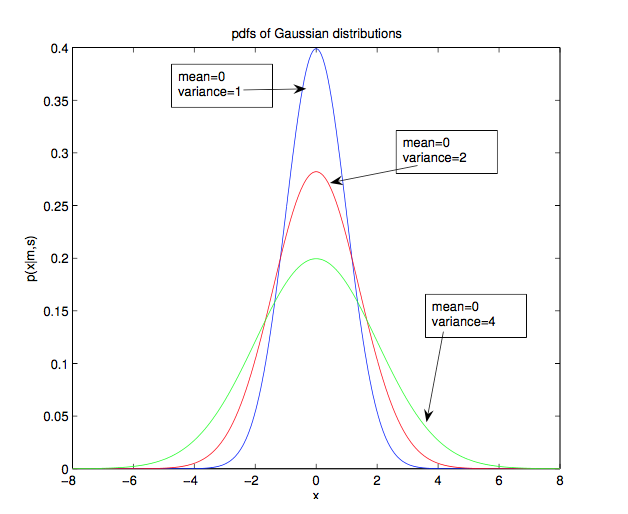
\includegraphics[width=0.5\linewidth]{figures/gmm.png}
\caption{pdfs of Gaussian distributions[7]}
\label{fig:gmm}
\end{figure}

  
  
  
\subsection{Hidden Markov Model}
The Hidden Markov Model \cite{Reference15}(HMM) is a popular statistical tool in process of speech recognition, since it can model a wide range of time series data and work on both audio and video frames. We use HMM in this project, which aims to recognize the extracted audio and video features as a series of HMM state. 


\begin{figure}[ht]
\centering
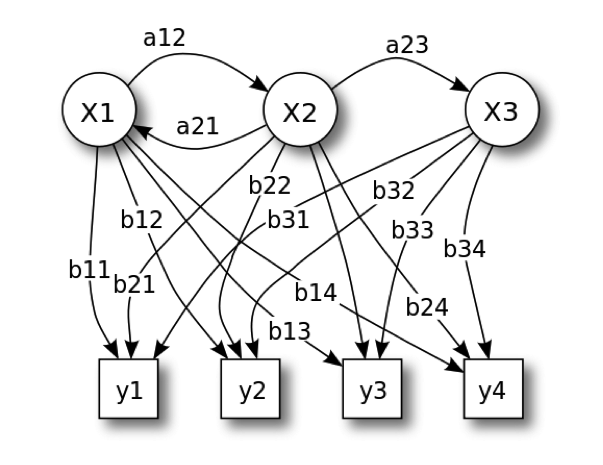
\includegraphics[width=0.5\linewidth]{figures/hmm.png}
\caption{Probabilistic parameters of a hidden Markov model}
\label{fig:hmm}
\end{figure}



As the figure \ref{fig:hmm} shows above, a HMM is composed by a sequence of states (x) that generates a sequence of emissions (y). And for states, there is a GMM probability density function (b) associated with each of them and also a transition probability (a) between them.  In addition, we can apply some basic training algorithms in HMM for maximum likelihood estimation to get the emissions. For Viterbi Algorithm\cite{Reference16}, it can be used to find the most likely path of getting the emissions without problems of hidden states. And for Forward Algorithm, we use it to compute the probability of the observation sequence after a given HMM. Besides, a combined version, forward-backward algorithm (Baum-Welch algorithm), can be adapted to estimate a most suitable HMM according to observed emissions with a related set of hidden states.

\subsection{Deep Neural Networks }
The neural network is a set of algorithms designed for mimicking the way that human brain works. Different with traditional machine learning algorithms, it can automatically extract features from unstructured data like audio and video frames and then cluster and classify them. Any particular Neural Networks like RNN or CNN are superposed by multiply layers while each layer composed by neural unit. Applied with an activation function, here is a figure\ref{fig:nn} shows how a neural unit, which from an input layer xi and weighted by a wi factor, that works.
\begin{figure}[ht]
\centering
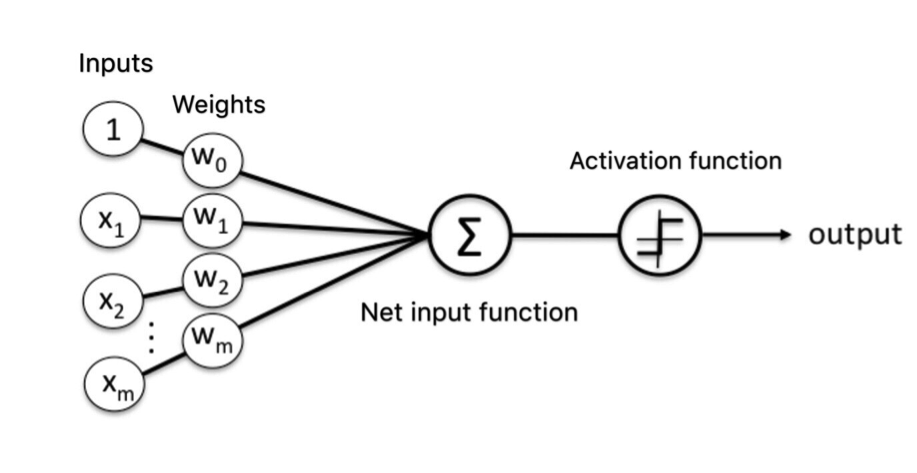
\includegraphics[width=0.5\linewidth]{figures/nn.png}\\[1cm]
\caption{neural unit work in neural networks}
\label{fig:nn}
\end{figure}




Besides, when it comes to DNN, there are at least 3 layers: input layer, hidden layer and output layer. Moreover, every layer learns on the basic of the former layer. Therefore, the future recognized by neural unit becomes complicated along with the increasing number of layers. 
Here is an example \ref{fig:dnn} to show the process of successive model layers learn deeper intermediate representations.
\begin{figure}[ht]
\centering
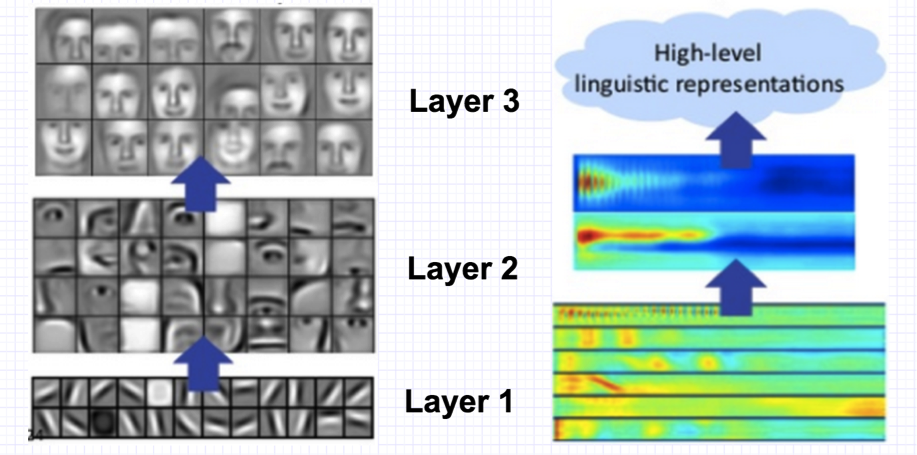
\includegraphics[width=1\linewidth]{figures/dnn.png}
\caption{the process of successive model layers learn deeper intermediate representations}
\label{fig:dnn}
\end{figure}

And to our project, the temporal aspect is important to both audio and video component. As a result, we feed the representation of each audio or video “frames” to a RNN in order to understand the sequential information between them, since a RNN is designed for recognizing sequences.  And especially use LSTM
to propagate and learn to control the informative streams over more time steps with forget gates. What is more, the CNN can be used to describe any individual frame and extract feature from them.

\section{HMM-GMM based ASR system in music}
Automatic Speech Recognition is a task to let machine learn how to convert the input signal into corresponded text.  And in this project, we adapt a traditional HMM-GMM statistic model into our systems. As the picture \ref{fig:hmmgmm} shows, HMM is to describe the dynamism with short-term stationary of states, and GMM describes the feature distribution in every state.
\begin{figure}[ht]
\centering
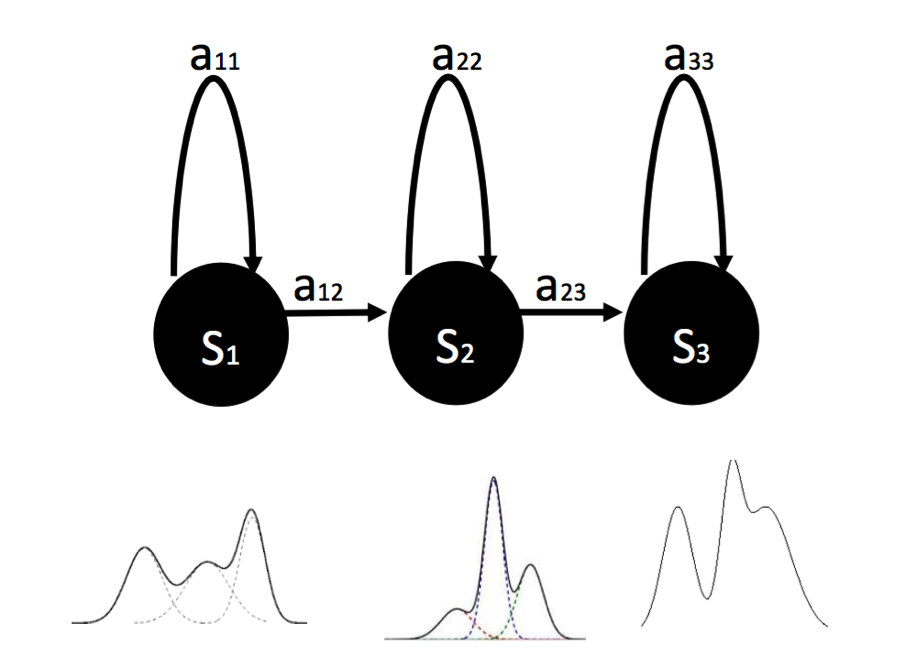
\includegraphics[width=0.5\linewidth]{figures/hmmgmm.png}
\caption{states in GMM-HMM}
\label{fig:hmmgmm}
\end{figure}
HMM-GMM based ASR systems also have mathematic framework of them stated as below: 
        \begin{equation}
        W^{*}=arg max P(W|X)
       =arg max\frac{P(X|W)P(W)}{P(X)}
       =arg max P(X|W)P(W)
        \end{equation} 
        
W represents transcription and X represents the input signal. For X is the input signal, it is hard to calculate the formula in the first line. Therefore, we adapt bayes formula in the second line. And for the input signals are continuous, the equation can be transformed into the third line.  At last, we need to find the most likely transcription W*. The HMM mathematic framework describes the process of an ASR system, w* represents the decode result, P (X|W) represents acoustic model and P (W) represents the language model. 
Moreover, words can be divided into sequences of HMM states Q. 
           
\subsection{Acoustic model}    
Refers to the equation above,the task of acoustic model is to compute P(X|W). No matter in audio ASR system or video ASR system, we both need to adapt their features to train acoustic models. In this project, we would train mono phone acoustic model and tri-phone acoustic model and compare their performances. 

As the figures \ref{fig:wsm} show below, the process of training acoustic models is to model the phones with HMMs, and the states of phones are presented in normal distribution. The system would update the parameters of HMM and GMM by iterated training.
        
\begin{figure}[ht]
\centering
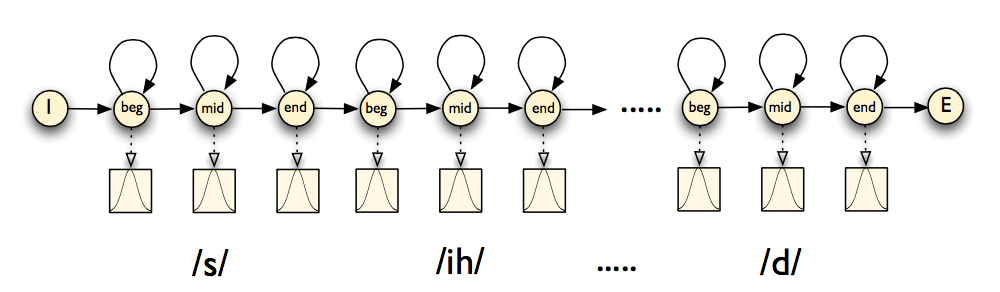
\includegraphics[width=1\linewidth]{figures/wsm.png}
\caption{'six quid' Word sequence models}
\label{fig:wsm}
\end{figure}

\subsection{Language model}
The language model represents the prior probability of the word sequence P(W) and is used for disambiguating between similar acoustics. For example, ‘ I want to see/sea ’. ‘Sea’ has the same pronunciation with ‘see’, but ‘I want to sea’ does not match the grammar rules.
And in speech recognition, language model are statistical model and usually be called as n-gram language model. On average, bigram is the most popular size of language model implemented in ASR system. However, it depends by different system’s database and would affect the system’s evaluation. We should decide the n-gram size by comparing system’s result. 

\subsection{Decode ASR systems}
In HMM-GMM based ASR systems, the developing process is mainly divided into 3 steps: feature extraction, classifier training, and decoding. Since the former two topics already been covered in former sections, this section is going to refer to the topic of decoding our ASR systems.
To show it clearly, here is the figure \ref{fig:aasr} and \ref{fig:vasr} to show the systems construction.
\begin{figure}[ht]
\centering
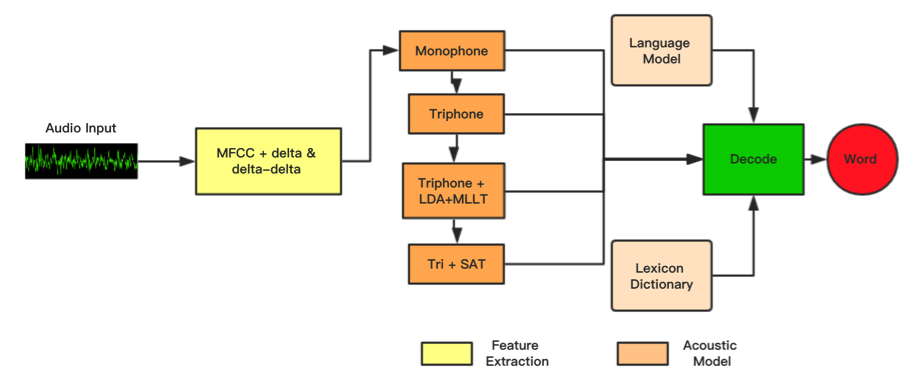
\includegraphics[width=1\linewidth]{figures/aasr.png}
\caption{audio-only ASR system construction}
\label{fig:aasr}
\end{figure}
\begin{figure}[ht]
\centering
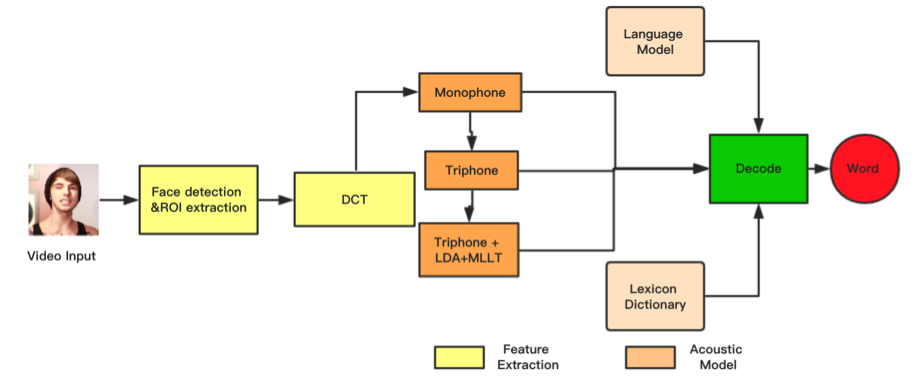
\includegraphics[width=1\linewidth]{figures/vasr.png}
\caption{visual-only ASR system construction}
\label{fig:vasr}
\end{figure}

In our system which is implemented in Kaldi, it would use OpenFst library to let all the resources of language model, acoustic model and grammar files are presented into fst format and generate decoding graph from them. At last, use viterbi algorithm to search the most likely path. 

\subsection{Dataset}
\subsubsection{Speech Database VS Singing Database}
Speech database is a database that concludes speech audio files and text transcription, while singing database composed by singing audio files and lyrics transcription. The singing voice is an artistic expression of speech voice spoken by singer, carrying with more information on musicality. While the speech voice tends to focus on completing the spoken word. On the other hand, the speech voice is flexible to change the pitch and loudness. But for singing voice, the frequencies fluctuate in a significantly soft way compared with speech voice. Moreover, the format of transcription between them is obviously different in the scope of topics and grammar. Text transcription may refer to any topics with a wide range and write with complicated grammar. But for lyrics transcription, the topics of it are limited. For example, probably no one would translate a science manuscript into a singing voice, while a speech voice is possible. What is more, the lyrics transcription usually has picky grammar like poems.
Thus, in terms of practicability, speech database are more suitable than singing database for no matter audio-only ASR system or AV-ASR system.

\section{summary}
To conclude this chapter, we mainly refer to the literature survey on the method of feature extraction, classification and components in ASR systems. They are all useful surveys of helping to build our ASR systems with HMM-GMM methodologies. However, to keep up the pace with the Lip-reading development nowadays, we should focus more on studying deep learning method to see whether it would improve the ASR system in music. Because no matter audio-only system or visual-only system is hard to get a good result in music with HMM-GMM methods.
The first end-to-end model, LipNet[8], which is learnt from deep learning methods, comes out last year. This breaking news can be said as a milestone event in the history of lip-reading research and also accelerate the development on these researches. However, even when the researches on lip-reading are emerging nowadays, Lip-reading for song transcription is still a barely analyzed issue. Therefore, this topic still has much space to exploit on it.
